    \begin{align}
	    \vec{n} &= \myvec{-1\\2+\sqrt{3}}
        \label{eq:11/10/2/4normal-vec}
	\\
	    \implies
        \implies \vec{n}^\top\vec{x} = \vec{n}^\top\vec{A} &= 4\brak{\sqrt{3}+1} \\
        \implies \myvec{-1&2+\sqrt{3}}\vec{x} &=\myvec{-1&2+\sqrt{3}}\myvec{2\\2\sqrt{3}}  
	    \\
	    &= 4\brak{\sqrt{3}+1}
        \label{eq:11/10/2/4line}
    \end{align}
is the desired equation.  See \figref{fig:11/10/2/4line}.
    \begin{figure}[!ht]
        \centering
        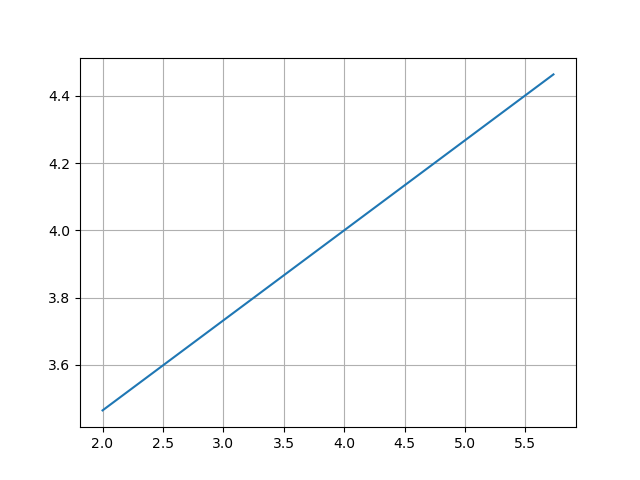
\includegraphics[width=\columnwidth]{chapters/11/10/2/4/figs/line.png}
        \caption{}
        \label{fig:11/10/2/4line}
    \end{figure}
